%Version 3.1 December 2024
% See section 11 of the User Manual for version history

%%%%%%%%%%%%%%%%%%%%%%%%%%%%%%%%%%%%%%%%%%%%%%%%%%%%%%%%%%%%%%%%%%%%%%
%%                                                                 %%
%% Please do not use \input{...} to include other tex files.       %%
%% Submit your LaTeX manuscript as one .tex document.              %%
%%                                                                 %%
%% All additional figures and files should be attached             %%
%% separately and not embedded in the \TeX\ document itself.       %%
%%                                                                 %%
%%%%%%%%%%%%%%%%%%%%%%%%%%%%%%%%%%%%%%%%%%%%%%%%%%%%%%%%%%%%%%%%%%%%%

%%\documentclass[referee,sn-basic]{sn-jnl}% referee option is meant for double line spacing

%%=======================================================%%
%% to print line numbers in the margin use lineno option %%
%%=======================================================%%

%%\documentclass[lineno,pdflatex,sn-basic]{sn-jnl}% Basic Springer Nature Reference Style/Chemistry Reference Style

%%=========================================================================================%%
%% the documentclass is set to pdflatex as default. You can delete it if not appropriate.  %%
%%=========================================================================================%%

%%\documentclass[sn-basic]{sn-jnl}% Basic Springer Nature Reference Style/Chemistry Reference Style

%%Note: the following reference styles support Namedate and Numbered referencing. By default the style follows the most common style. To switch between the options you can add or remove �Numbered� in the optional parenthesis.
%%The option is available for: sn-basic.bst, sn-chicago.bst%

\documentclass[pdflatex,sn-nature]{sn-jnl}% Style for submissions to Nature Portfolio journals
%\documentclass[pdflatex,sn-basic]{sn-jnl}% Basic Springer Nature Reference Style/Chemistry Reference Style
%\documentclass[pdflatex,sn-mathphys-num]{sn-jnl}% Math and Physical Sciences Numbered Reference Style
%\documentclass[pdflatex,sn-mathphys-ay]{sn-jnl}% Math and Physical Sciences Author Year Reference Style
%\documentclass[pdflatex,sn-aps]{sn-jnl}% American Physical Society (APS) Reference Style
%\documentclass[pdflatex,sn-vancouver-num]{sn-jnl}% Vancouver Numbered Reference Style
%\documentclass[pdflatex,sn-vancouver-ay]{sn-jnl}% Vancouver Author Year Reference Style
%\documentclass[pdflatex,sn-apa]{sn-jnl}% APA Reference Style
%\documentclass[pdflatex,sn-chicago]{sn-jnl}% Chicago-based Humanities Reference Style

%%%% Standard Packages
%%<additional latex packages if required can be included here>

\usepackage{graphicx}%
\usepackage{multirow}%
\usepackage{amsmath,amssymb,amsfonts}%
\usepackage{amsthm}%
\usepackage{mathrsfs}%
\usepackage[title]{appendix}%
\usepackage{xcolor}%
\usepackage{textcomp}%
\usepackage{manyfoot}%
\usepackage{booktabs}%
\usepackage{algorithm}%
\usepackage{algorithmicx}%
\usepackage{algpseudocode}%
\usepackage{listings}%

\usepackage{standalone}
\usepackage{tikz}
\usepackage[dvipsnames]{xcolor}
\usepackage{geometry}

% Minted package for beautiful syntax highlighting
\usepackage{minted}
\usemintedstyle{borland}
\setminted{
  fontsize=\small,
  breaklines=true,
  autogobble,
  frame=single,
  framesep=2mm,
  linenos
}

% Use bash lexer for TSG code examples (since it handles # comments well)
\newminted{bash}{
  fontsize=\small,
  breaklines=true,
  autogobble,
  frame=single,
  framesep=2mm,
  linenos
}

% Define a standard environment for TSG code (using \newenvironment instead of \renewenvironment)
\newenvironment{tsgcode}
  {\VerbatimEnvironment\begin{minted}[fontsize=\small,breaklines=true,autogobble,frame=single,framesep=2mm,linenos]{bash}}
  {\end{minted}}

\usetikzlibrary{shadows,shapes,arrows,positioning,fit,backgrounds,decorations.pathreplacing,calc}

\graphicspath{{../figures}}

\usepackage[acronym, automake, style=index, shortcuts]{glossaries-extra}
\setabbreviationstyle[acronym]{long-short}
% define glossaries
\makeglossaries

\newacronym{gpu}{GPU}{Graphics Processing Unit}
\newacronym{hpc}{HPC}{High Performance Computing}

\newacronym{ide}{IDE}{Integrated Development Environment}
\newacronym{cd}{CD}{Continuous Development}
\newacronym{ucsc}{UCSC}{UCSC Genome Browser}
\newacronym{glm}{GLM}{Genomic Language Model}
\newacronym{lcglm}{LCGLM}{long-context genomic language model}
\newacronym{snp}{SNP}{Single Nucleotide Polymorphism}

\newacronym{mlp}{MLP}{multilayer perceptron}
\newacronym{drs}{dRNA-seq}{direct RNA sequencing}
\newacronym{ont}{ONT}{Oxford Nanopore Technologies}
\newacronym{pb}{PacBio}{Pacific Biosciences}

\newacronym{tsg}{TSG}{Transcriptome Segment Graph}
\newacronym{nlt}{NLT}{Non-colinear Transcript}

\newacronym{go}{GO}{Gene Ontology}
\newacronym{pcr}{PCR}{Polymerase Chain Reaction}
\newacronym{mrna}{mRNA}{messenger RNA}

%%%%%=============================================================================%%%%
%%%%  Remarks: This template is provided to aid authors with the preparation
%%%%  of original research articles intended for submission to journals published
%%%%  by Springer Nature. The guidance has been prepared in partnership with
%%%%  production teams to conform to Springer Nature technical requirements.
%%%%  Editorial and presentation requirements differ among journal portfolios and
%%%%  research disciplines. You may find sections in this template are irrelevant
%%%%  to your work and are empowered to omit any such section if allowed by the
%%%%  journal you intend to submit to. The submission guidelines and policies
%%%%  of the journal take precedence. A detailed User Manual is available in the
%%%%  template package for technical guidance.
%%%%%=============================================================================%%%%

%% as per the requirement new theorem styles can be included as shown below
\theoremstyle{thmstyleone}%
\newtheorem{theorem}{Theorem}%  meant for continuous numbers
%%\newtheorem{theorem}{Theorem}[section]% meant for sectionwise numbers
%% optional argument [theorem] produces theorem numbering sequence instead of independent numbers for Proposition
\newtheorem{proposition}[theorem]{Proposition}%
%%\newtheorem{proposition}{Proposition}% to get separate numbers for theorem and proposition etc.

\theoremstyle{thmstyletwo}%
\newtheorem{example}{Example}%
\newtheorem{remark}{Remark}%

\theoremstyle{thmstylethree}%
\newtheorem{definition}{Definition}%

\raggedbottom
%%\unnumbered% uncomment this for unnumbered level heads

\begin{document}

\title[Article Title]{ChimeraLM: A genomic language model to detect chimer artifa}

%%=============================================================%%
%% GivenName	-> \fnm{Joergen W.}
%% Particle	-> \spfx{van der} -> surname prefix
%% FamilyName	-> \sur{Ploeg}
%% Suffix	-> \sfx{IV}
%% \author*[1,2]{\fnm{Joergen W.} \spfx{van der} \sur{Ploeg}
%%  \sfx{IV}}\email{iauthor@gmail.com}
%%=============================================================%%
\author[1]{\fnm{Yangyang} \sur{Li}}\email{yangyang.li@northwestern.edu}
% \equalcont{These authors contributed equally to this work.}

% \author*[1,2]{\fnm{First} \sur{Author}}\email{iauthor@gmail.com}
% \author[1]{\fnm{Ting-You} \sur{Wang}}\email{tywang@northwestern.edu}
% \equalcont{These authors contributed equally to this work.}

% \author[1]{\fnm{Qingxiang} \sur{Guo}}\email{qingxiang.guo@northwestern.edu}
\author*[1,2]{\fnm{Rendong} \sur{Yang}}\email{rendong.yang@northwestern.edu}

\affil[1]{\orgdiv{Department of Urology}, \orgname{Northwestern University Feinberg School of Medicine}, \orgaddress{\street{303 E Superior St}, \city{Chicago}, \postcode{60611}, \state{IL}, \country{USA}}}
\affil[2]{\orgdiv{Robert H. Lurie Comprehensive Cancer Center}, \orgname{Northwestern University Feinberg School of Medicine}, \orgaddress{\street{675 N St Clair St}, \city{Chicago}, \postcode{60611}, \state{IL}, \country{USA}}}

\abstract{
	\gls{nlt} arising from structural variations challenge conventional linear analysis approaches in transcriptomics.
	Here we introduce the concept of \gls{tsg} and present the first comprehensive infrastructure for graph-based transcript analysis.
	We develop the TSG file format as the first standardized encoding for transcript segment graphs, enabling systematic representation of \gls{nlt}, and complex splicing patterns impossible to capture with linear methods.
	Our command-line toolkit provides the first comprehensive suite for \gls{tsg} manipulation, analysis, and format conversion, while Aurora offers the first interactive visualization platform for transcript segment graphs.
	Together with our companion TSG caller scannls, this work establishes the foundational infrastructure for a new paradigm in transcriptomic analysis, providing the essential tools for systematic investigation of \gls{nlt} structures.
}
\keywords{Transcriptomics, Graph-based analysis, Non-colinear transcripts, TSG caller, TSG visualization}

%%\pacs[JEL Classification]{D8, H51}
%%\pacs[MSC Classification]{35A01, 65L10, 65L12, 65L20, 65L70}

\maketitle

\section{main}\label{sec1}

Transcriptomic structural variations, including gene fusions, circular RNAs, and complex alternative splicing, play critical roles in cancer, development, and disease.

% \begin{figure}
% 	\begin{center}
% 		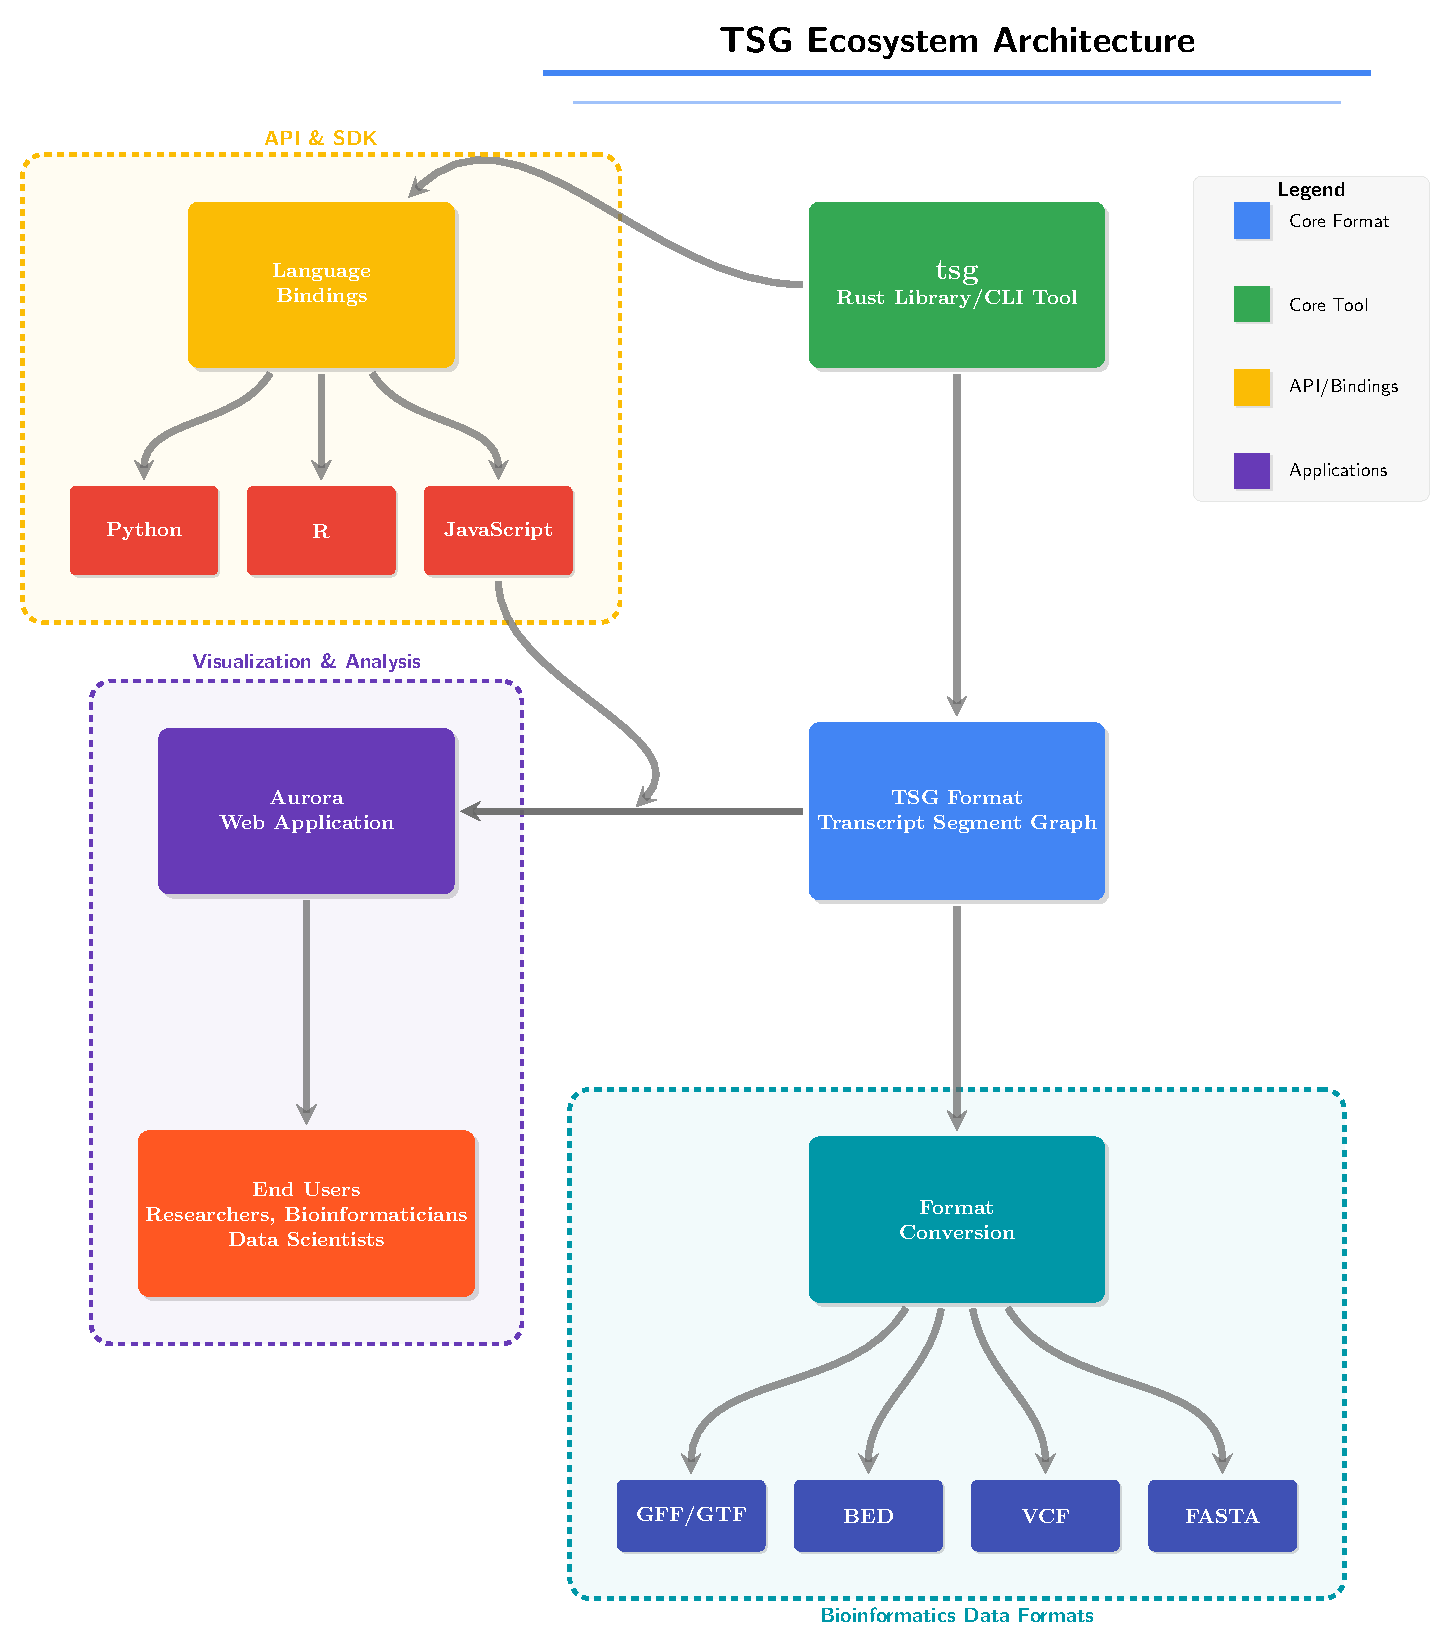
\includegraphics[width=0.95\textwidth]{figures/figure1}
% 	\end{center}
% 	\caption{TSG Ecosystem}\label{fig:figure1}
% \end{figure}

\section{Methods}\label{sec11}

Topical subheadings are allowed. Authors must ensure that their Methods section includes adequate experimental and characterization data necessary for others in the field to reproduce their work. Authors are encouraged to include RIIDs where appropriate.

If your manuscript includes potentially identifying patient/participant information, or if it describes human transplantation research, or if it reports results of a clinical trial then  additional information will be required. Please visit (\url{https://www.nature.com/nature-research/editorial-policies}) for Nature Portfolio journals, (\url{https://www.springer.com/gp/authors-editors/journal-author/journal-author-helpdesk/publishing-ethics/14214}) for Springer Nature journals, or (\url{https://www.biomedcentral.com/getpublished/editorial-policies\#ethics+and+consent}) for BMC.

\backmatter

\bmhead{Supplementary information}

This separation aligns with how many transcript assembly algorithms work:

\begin{enumerate}[leftmargin=*]
	\item First, chains of exons and splice junctions are identified from the data
	\item Then, potential transcripts are derived by traversing the graph in different ways
	\item Finally, relationships between different transcript graphs are established
\end{enumerate}

\bmhead{Acknowledgements}

Acknowledgements are not compulsory. Where included they should be brief. Grant or contribution numbers may be acknowledged.

Please refer to Journal-level guidance for any specific requirements.

\section*{Declarations}

Some journals require declarations to be submitted in a standardised format. Please check the Instructions for Authors of the journal to which you are submitting to see if you need to complete this section. If yes, your manuscript must contain the following sections under the heading `Declarations':

\begin{itemize}
	\item Funding
	\item Conflict of interest/Competing interests (check journal-specific guidelines for which heading to use)
	\item Ethics approval and consent to participate
	\item Consent for publication
	\item Data availability
	\item Materials availability
	\item Code availability
	\item Author contribution
\end{itemize}

\noindent
If any of the sections are not relevant to your manuscript, please include the heading and write `Not applicable' for that section.

\begin{flushleft}%
	Editorial Policies for:
	
	\bigskip\noindent
	Springer journals and proceedings: \url{https://www.springer.com/gp/editorial-policies}
	
	\bigskip\noindent
	Nature Portfolio journals: \url{https://www.nature.com/nature-research/editorial-policies}
	
	\bigskip\noindent
	\textit{Scientific Reports}: \url{https://www.nature.com/srep/journal-policies/editorial-policies}
	
	\bigskip\noindent
	BMC journals: \url{https://www.biomedcentral.com/getpublished/editorial-policies}
\end{flushleft}

\begin{appendices}

	\section{Section title of first appendix}\label{secA1}
	
	An appendix contains supplementary information that is not an essential part of the text itself but which may be helpful in providing a more comprehensive understanding of the research problem or it is information that is too cumbersome to be included in the body of the paper.
	
	%%=============================================%%
	%% For submissions to Nature Portfolio Journals %%
	%% please use the heading ``Extended Data''.   %%
	%%=============================================%%
	
	%%=============================================================%%
	%% Sample for another appendix section			       %%
	%%=============================================================%%
	
	%% \section{Example of another appendix section}\label{secA2}%
	%% Appendices may be used for helpful, supporting or essential material that would otherwise
	%% clutter, break up or be distracting to the text. Appendices can consist of sections, figures,
	%% tables and equations etc.
	
\end{appendices}

%%===========================================================================================%%
%% If you are submitting to one of the Nature Portfolio journals, using the eJP submission   %%
%% system, please include the references within the manuscript file itself. You may do this  %%
%% by copying the reference list from your .bbl file, paste it into the main manuscript .tex %%
%% file, and delete the associated \verb+\bibliography+ commands.                            %%
%%===========================================================================================%%

\bibliography{sn-bibliography}% common bib file
%% if required, the content of .bbl file can be included here once bbl is generated
%%\input sn-article.bbl

\end{document}
